\begin{frame}{Composites}
    % Thesis repository \texttt{dock/thesis/figures/design/model/presentation.pdf}
    \begin{itemize}
        \item A composite is a template that describes high-level logical components
        \begin{itemize}
            \item It can be of two types:
            \begin{itemize}
                \item Server (e.g., “web server”, “database”, ...)
                \item INP (e.g., “IncBricks caching system”, “NetChain locking system”, ...)
            \end{itemize}
            \item It can be made out of
            \begin{itemize}
                \item Other Composites
                \begin{description}[abc] % for indentation of length of abc
                    \item[$\bullet$] A composite loop must not be valid, since it would be impossible to place % FIXME
                \end{description}
                \item Logical resources
            \end{itemize}
        \end{itemize}
    \end{itemize}
\end{frame}

\begin{frame}{The extended-Tenant Application Graph (eTag)}
    % \begin{itemize}
    %     \item (5.2.1 why existing resource models do not satisfy all requirements)
    %     \item (5.2.2 eTag)
    % \end{itemize}
    \centering
    \includegraphics[page=3, clip, trim=0.6cm 0.6cm 0.6cm 0.6cm, width=\textwidth]{design/model/variants.pdf}
\end{frame}

\begin{frame}{The template database}
    \begin{itemize}
        \item (5.3 generic groups)
        \item (5.1.2 template database role)(5.1.2 template database role)
    \end{itemize}
\end{frame}

\begin{frame}{Mapping composites to logical resources}
    \begin{itemize}
        \item Composites must be translated into logical resources
        \item This is done using the template database managed by the RM
        \begin{center}
            \includegraphics[page=4, clip, trim=4.3cm 0.2cm 4.3cm 7.65cm, width=0.95\textwidth]{design/model/presentation.pdf}
        \end{center}
    \end{itemize}
\end{frame}

\begin{frame}{Placing logical resources}
    \begin{columns}[T,onlytextwidth]
        \column{0.3\textwidth}
        \begin{itemize}
            \item The placement algorithm places logical resource onto physical ones
            \item Three types of physical resources:
            \begin{itemize}
                \item Server
                \item Switch
                \item Link
            \end{itemize}
        \end{itemize}
        \column{0.7\textwidth}
        \includegraphics[page=5, clip, trim=11.2cm 3.7cm 0.6cm 3.6cm, width=\textwidth]{design/model/presentation.pdf}
    \end{columns}
\end{frame}

\begin{frame}{1\textsuperscript{st} approach: passive template mapping}
    \centering
    \includegraphics[page=7, clip, trim=3.75cm 1.05cm 3.05cm 3.8cm, width=\textwidth]{design/model/presentation.pdf}
\end{frame}

\begin{frame}{2\textsuperscript{nd} approach: active template mapping}
    \centering
    \includegraphics[page=8, clip, trim=2.1cm 1.95cm 1.8cm 4.1cm, width=\textwidth]{design/model/presentation.pdf}
\end{frame}

\begin{frame}{The whole picture}
    \centering
    \includegraphics[page=6, clip, trim=0.35cm 2.1cm 0.35cm 5cm, width=1\textwidth]{design/model/presentation.pdf}
\end{frame}

\begin{frame}{Generic groups?} % FIXME
\end{frame}
